\textbf{COLUNI 2026 -- Questão 27}\par\medskip No filme \textit{Lilo e Stitch}, nova animação da Disney de 2025, Stitch é uma forma de vida extraterrestre geneticamente modificada. Possui pelagem azul com o corpo semelhante ao de um coala. Stitch chega ao planeta Terra após fugir de sua prisão e tenta se passar por um cachorro como mostrado no filme.

Os cachorros são mamíferos e, como tal, apresentam um conjunto de características comum a esse grupo de animais.

\begin{figure}[htbp]
\centering
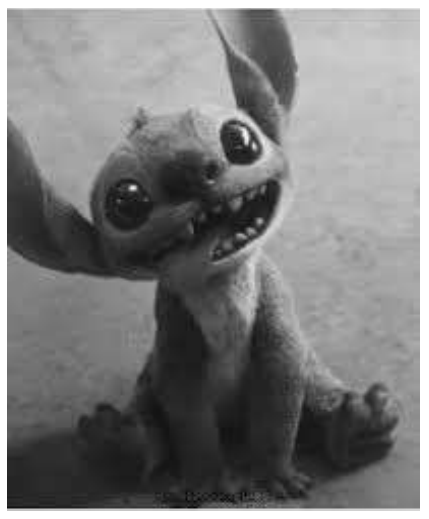
\includegraphics[width=0.40\linewidth]{static/simulados/coluni/figuras/2026/questao-27/figura-1.png}
\end{figure}

Disponível em: https://ingresso.com. Acesso em: 19 ago. 2025.

Das características abaixo, assinale aquela que NÃO deve ser utilizada por Stitch, pois não está presente nos cachorros e, portanto, não ajudará em seu disfarce.\begin{enumerate}
\item Pele como órgão de revestimento e proteção, desprovida de glândulas e com importantes funções sensoriais.
\item Sistema circulatório com vasos sanguíneos, sangue e coração com quatro câmaras cardíacas.
\item Variação nos tipos de dentes, com caninos desenvolvidos, diferenciando dos incisivos e dos molares.
\item Condição endotérmica com pelos recobrindo o corpo e uma grossa camada de gordura abaixo da pele.\end{enumerate}